\documentclass[11pt,a4paper]{article}

\usepackage[margin=2.0cm]{geometry}
\usepackage{amsmath,amssymb,amsfonts}
\usepackage[T1]{fontenc}
\usepackage{lmodern}
\usepackage{microtype}
\usepackage{enumitem}
\usepackage{booktabs}
\usepackage{tabularx}
\usepackage{xcolor}
\usepackage[hidelinks,colorlinks=true,
            urlcolor=blue!50!black,
            linkcolor=blue!50!black,
            citecolor=blue!50!black]{hyperref}
\usepackage{listings}
\usepackage{tikz}
\usetikzlibrary{positioning,arrows.meta,shapes.geometric,fit,calc}

\definecolor{matclr}{RGB}{40,103,160}
\definecolor{unitclr}{RGB}{180,70,40}
\definecolor{rawclr}{RGB}{50,140,80}
\definecolor{prodclr}{RGB}{160,60,140}
\definecolor{kept}{RGB}{40,140,80}
\definecolor{cut}{RGB}{170,60,60}
\definecolor{accent}{RGB}{200,120,30}

\tikzset{
    mat/.style={circle,draw=matclr,thick,fill=matclr!10,
                minimum size=8mm,inner sep=1pt,font=\small},
    raw/.style={mat,draw=rawclr,fill=rawclr!12},
    prod/.style={mat,draw=prodclr,fill=prodclr!12,line width=0.6mm},
    unit/.style={rectangle,draw=unitclr,thick,fill=unitclr!10,
                  minimum height=8mm,minimum width=12mm,
                  rounded corners=1pt,inner sep=2pt,font=\small},
    edge/.style={-{Stealth[length=2.2mm]},semithick},
    kept/.style={fill=kept!18},
    cut/.style ={fill=cut!18,opacity=0.7},
}

\lstset{
    basicstyle=\ttfamily\footnotesize,
    breaklines=true,
    columns=fullflexible,
    keepspaces=true,
    showstringspaces=false,
    xleftmargin=0pt,xrightmargin=0pt,
    frame=single,
    rulecolor=\color{gray!30},
}

\newcommand{\HyMeKo}{\textsc{HyMeKo}}
\newcommand{\code}[1]{\texttt{\small #1}}
\setlist[itemize]{leftmargin=1.4em,itemsep=2pt,topsep=3pt}
\setlist[enumerate]{leftmargin=1.6em,itemsep=2pt,topsep=3pt}

\title{ABB / SSG / MSG in \HyMeKo:\\[4pt]
       \large\normalfont objective, numbers, and chemical-process use}
\author{Dossier for Jean Pimentel\\
        \small Pannonia / P-graph community}
\date{2026-05-18}

\begin{document}
\maketitle

\begin{abstract}
\noindent
This summary collects the state of the Friedler P-graph machinery
inside the \HyMeKo{} signed-hypergraph framework, addressing three
questions raised by Pimentel: (i) what is the multi-objective form
used in our ABB / SSG / MSG and what governing rule selects branches,
(ii) what numerical results have we obtained for both optimisation
and pruning, and (iii) what chemical-process and raw-chemical-feedstock
use cases the same machinery supports. The codebase contains two ABB
layers --- a direct Friedler-Tarj\'an-Huang-Fan 1992 reproduction over
P-graph operating units, and a structural generalisation to signed-cycle
enumeration that exposes a nestable weighted-sum multi-objective.
The empirical contribution is a graph-property-conditional
axiom-selection rule (best pruner depends on a structural ratio), with
direct analogue to feedstock-conditional unit selection in PSE.
\end{abstract}

\section{Two ABB layers in one codebase}

The codebase implements \emph{two} distinct accelerated branch-and-bound
(ABB) algorithms that share the same axiom + bound + DFS structure.
The first is the direct P-graph descendant; the second is the
generalisation we use for signed-cycle enumeration. Both are useful
for the PSE community; the multi-objective form lives in the second.

\paragraph{Layer 1 --- P-graph ABB.} Module \code{hymeko\_pgraph::abb}.
Direct reproduction of Friedler, Tarj\'an, Huang \& Fan (1992) over a
\code{LoweredPGraph} $(M, O, E_{\text{dir}}, R, P, c)$ with materials
$M$, operating units $O$, directed bipartite edges $E_{\text{dir}}$,
raw set $R \subseteq M$, product demand $P \subseteq M$, and per-unit
cost $c: O \to \mathbb{R}_{\geq 0}$.

\paragraph{Layer 2 --- Cycle-enumeration ABB.} Module
\code{hymeko\_graph::topk\_cycles}. Selects the top-$K$ closed cycles
of length $k$ from a signed graph under a \emph{\code{BoundedScorer}
trait}. The trait exposes a per-cycle score and an admissible upper
bound on that score given the partial DFS path.

The unifying mental model:

\begin{center}\small
\begin{tabular}{p{0.42\linewidth}l p{0.42\linewidth}}
\toprule
P-graph layer & & Cycle-enum layer \\
\midrule
Operating unit $u \in O$           &  $\leftrightarrow$ &  DFS extension by one edge \\
Cost $c(u)$                        &  $\leftrightarrow$ &  Per-cycle score $s(\text{cycle})$ \\
Material reachability $C_R(O')$    &  $\leftrightarrow$ &  BFS reachability from start vertex \\
Demand set $P$                     &  $\leftrightarrow$ &  Heap fill target $K$ \\
Inclusion bound                    &  $\leftrightarrow$ &  Score UB $\leq$ heap threshold \\
Reachability bound                 &  $\leftrightarrow$ &  BFS distance $>$ $k_{\text{remaining}}$ \\
MSG forward/backward trim          &  $\leftrightarrow$ &  Per-start BFS pre-pass \\
SSG bitmask enumeration            &  $\leftrightarrow$ &  (replaced by the size-$K$ heap) \\
\bottomrule
\end{tabular}
\end{center}

\section{Multi-objective function and governing rule}

\subsection{P-graph layer --- single-criterion cost minimisation}

The Layer-1 objective is a scalar cost minimisation:
\[
\boxed{\;
\min_{O' \subseteq O_{\max}}\; \sum_{u \in O'} c(u)\;
\;\text{s.t.}\;
\begin{cases}
\forall u \in O',\ \mathrm{in}(u) \subseteq C_R(O') & \text{(input consistency)}\\
P \subseteq C_R(O') & \text{(demand)}\\
\text{every non-raw, non-product output is consumed} & \text{(no-excess, strict)}
\end{cases}\;}
\]
where $C_R(O')$ is the producibility closure (least fixed point starting
from $R$, adding $\mathrm{out}(u)$ for every $u \in O'$ whose inputs lie
already in the set).

\paragraph{Governing rule: two bounds + DFS branching.}
\begin{itemize}
\item \textbf{Inclusion bound}: abandon a partial selection whose
      accumulated cost has reached or exceeded the current
      incumbent's cost.
\item \textbf{Reachability bound}: let
      $\widehat{O} = \text{included} \cup \text{undecided}$. If
      $C_R(\widehat{O}) \not\supseteq P$, no descendant can be
      feasible --- prune. This is the dominant pruner for sparse
      problems.
\end{itemize}
Branching order is fixed; each step takes \emph{include before exclude}
so a feasible incumbent appears early and the inclusion bound fires
fast (\code{hymeko\_pgraph/src/abb.rs:119--180}).

\textbf{MSG} (Maximal Structure Generation) is the preprocessing: iteratively
trim units that fail forward-feasibility (input set unreachable from
$R$) or backward-utility (output set not used by any other unit /
product). Reaches a fixpoint in $O(|O|)$ rounds; the output $O_{\max}$
is the largest \emph{potentially feasible} subset, and ABB explores
$2^{|O_{\max}|}$.

\textbf{SSG} (Solution Structure Generation) is the exhaustive companion:
enumerate every feasible $O' \subseteq O_{\max}$ instead of just the
minimum-cost one. Used when $|O_{\max}| \leq 30$; above that, ABB is
the right tool.

\subsection{Cycle-enumeration layer --- the multi-objective lives here}

The Layer-2 objective maximises a \emph{weighted sum} of per-cycle scores
via the \code{WeightedSumScorer<S1, S2>} type
(\code{hymeko\_graph/src/topk\_cycles.rs:2278}):
\[
\boxed{\;\mathrm{score}_{\mathrm{comp}}(c) = a \cdot s_1(c) + b \cdot s_2(c),
\qquad a, b \geq 0.\;}
\]
The admissible upper bound is the sum of admissible upper bounds:
\[
\mathrm{UB}_{\mathrm{comp}}(\text{partial})
   = a \cdot \mathrm{UB}_{s_1}(\text{partial})
   + b \cdot \mathrm{UB}_{s_2}(\text{partial})
   \;\geq\; \mathrm{score}_{\mathrm{comp}}(\text{any closed extension}).
\]
\code{WeightedSumScorer} is \emph{nestable}: \code{WeightedSum<WeightedSum<A,B>, C>}
gives a triple-criterion scalarisation, etc.

\paragraph{Atomic scorers.} Four \code{BoundedScorer} impls ship:
\begin{center}\small
\begin{tabular}{lll}
\toprule
Scorer & $s(\text{cycle})$ & Upper bound \\
\midrule
\code{FractionNegativeScorer} & $(\#\text{neg edges}) / k$ & $(n_{\text{neg so far}} + k_{\text{remaining}}) / k_{\text{len}}$ \\
\code{BalanceScorer} (Cartwright-Harary) & $\prod s_i \in \{-1, +1\}$ & $+1$ (closure can flip parity) \\
\code{SignProductAbsScorer}              & $|\prod s_i| = 1$         & $1$ \\
\code{LowRootScorer} & $-v_0$ (smallest start vertex) & $0$ (loose) \\
\bottomrule
\end{tabular}
\end{center}

\paragraph{Governing rule: score upper bound vs heap threshold.}
At each DFS extension from a partial path with $n_{\text{neg so far}}$
negative edges and $k_{\text{remaining}}$ edges left to close,
compute $\mathrm{UB}$. If $\mathrm{UB} \leq \texttt{heap.peek\_min()}$,
prune. Otherwise descend. Structurally identical to Layer 1's
inclusion bound, with ``cost $\geq$ incumbent'' replaced by
``score $\leq$ heap min'' (max-heap inversion). The reachability bound
is replaced by a per-start-vertex BFS pre-pass that rejects starts
whose neighbourhood cannot close a length-$k$ cycle.

\section{The HDA worked example (P-graph ABB)}

\subsection{Process and encoding}

HDA (hydrodealkylation of toluene): toluene $+$ H$_2$ $\to$ benzene
($+$ methane as by-product). Five materials, four operating units,
single product demand. In \HyMeKo{} grammar:

\begin{lstlisting}
HDA{} context {
    Toluene <material, raw>;   H2 <material, raw>;
    Mix <material>;
    Benzene <material, product>;   Methane <material>;

    @Mixer       <unit> 100 { (-Toluene, -H2, +Mix); }
    @Reactor     <unit> 250 { (-Mix, +Benzene, +Methane); }
    @DirectSynth <unit> 800 { (-Toluene, -H2, +Benzene); }
    @Disposal    <unit>  50 { (-Methane); }
}
\end{lstlisting}

\subsection{P-graph view}

\begin{center}
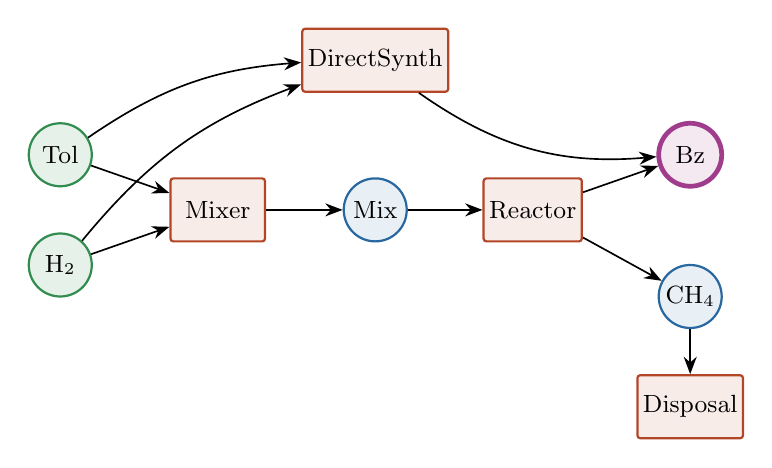
\begin{tikzpicture}[node distance=10mm and 14mm]
\node[raw] (T)   at (0,3.4) {Tol};
\node[raw] (H2)  at (0,2.0) {H$_2$};
\node[mat] (Mix) at (4.0,2.7) {Mix};
\node[prod](B)   at (8.0,3.4) {Bz};
\node[mat] (Me)  at (8.0,1.6) {CH$_4$};

\node[unit] (Mx) at (2.0,2.7) {Mixer};
\node[unit] (Rx) at (6.0,2.7) {Reactor};
\node[unit] (Ds) at (8.0,0.2) {Disposal};
\node[unit] (Dr) at (4.0,4.6) {DirectSynth};

\draw[edge] (T) -- (Mx);  \draw[edge] (H2) -- (Mx);
\draw[edge] (Mx) -- (Mix); \draw[edge] (Mix) -- (Rx);
\draw[edge] (Rx) -- (B);   \draw[edge] (Rx) -- (Me);
\draw[edge] (Me) -- (Ds);
\draw[edge,bend left=15] (T) to (Dr);
\draw[edge,bend left=15] (H2) to (Dr);
\draw[edge,bend right=20] (Dr) to (B);
\end{tikzpicture}
\end{center}

\subsection{Results table}

\begin{center}\small
\begin{tabular}{lll}
\toprule
Algorithm                 & Output                                     & Cost \\
\midrule
MSG                       & $\{$Mixer, Reactor, Disposal, DirectSynth$\}$ & --- \\
SSG (strict no-excess)    & $\{\{$Mx, Rx, Ds$\},\,\{$DS$\}\}$           & --- \\
SSG (relaxed)             & 4 structures incl.\ $\{$Mx, Rx$\}$          & --- \\
\textbf{ABB (strict)}     & $\{$Mixer, Reactor, Disposal$\}$            & \textbf{400} \\
ABB (relaxed)             & $\{$Mixer, Reactor$\}$                      & 350 \\
\bottomrule
\end{tabular}
\end{center}

\paragraph{Tree compression.} ABB explored \textbf{7 nodes vs the full
lattice $2^4 = 16$} --- 56\% killed before evaluation. The
\code{$\lnot$Mixer} branch dies at the reachability bound (Mix becomes
unreachable). The \code{$+$DirectSynth} branch is dominated by the
inclusion bound at $c = 800 > 400$.

\begin{center}
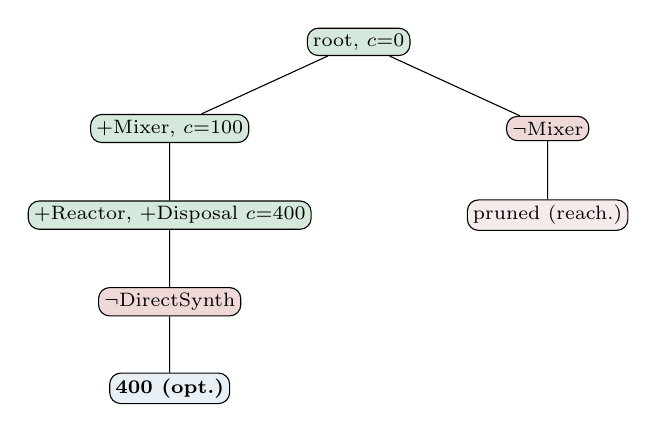
\begin{tikzpicture}[
    level distance=11mm,
    level 1/.style={sibling distance=48mm},
    every node/.style={font=\scriptsize},
    inc/.style={draw,fill=kept!20,rounded corners,inner sep=2pt},
    exc/.style={draw,fill=cut!20,rounded corners,inner sep=2pt},
    leaf/.style={draw,fill=matclr!10,rounded corners,inner sep=2pt},
    pr/.style={draw,fill=cut!10,rounded corners,inner sep=2pt},
]
\node[inc] {root, $c{=}0$}
  child {node[inc] {$+$Mixer, $c{=}100$}
    child {node[inc] {$+$Reactor, $+$Disposal $c{=}400$}
      child {node[exc] {$\lnot$DirectSynth}
        child {node[leaf] {\textbf{400 (opt.)}}}
      }
    }
  }
  child {node[exc] {$\lnot$Mixer}
    child {node[pr] {pruned (reach.)}}
  };
\end{tikzpicture}
\end{center}

\section{Cycle-ABB at production scale}

\subsection{The signed-cycle setting}

For each cycle of length $k$ in a signed graph, the cycle carries
the $k$ edge signs along its traversal. The Cartwright-Harary balance
$\prod_{i=1}^{k} s_i \in \{-1, +1\}$ tells you whether the cycle is
Heider-balanced. Real signed graphs (Bitcoin trust, Slashdot foes,
Epinions reviews) range from $\approx 95\%$ balanced (cooperative)
to $\approx 87\%$ balanced (adversarial with visible conflict).

Full cycle enumeration is intractable at scale: Slashdot at $k = 4$
contains \textbf{55.5 million} cycles ($\geq 8$~GB materialised).
The cycle-ABB layer compresses this to a per-vertex top-$m$
subset $|M_e| \leq |V| \cdot m$, a $50$--$150\times$ memory cut.

\subsection{Wall-time speedup}

Plan-driven benchmark on \textbf{Epinions} signed graph (131\,828
vertices, 840\,799 edges, 14.7\% negative), $k = 4$, $K = 10\,000$,
\code{CartwrightHararyPruner(OnlyBalanced)},
\code{FractionNegativeScorer}, 5-iteration measurement protocol per
CLAUDE.md \S 3:

\begin{center}\small
\begin{tabular}{lrrr}
\toprule
Path                                   & Median wall & IQR & Speedup \\
\midrule
Baseline (\code{enumerate\_top\_k\_cycles\_par})  & 100.557 s & 0.205 s & 1.00$\times$ \\
\textbf{ABB} (\code{...\_par\_bb})                & \textbf{4.012 s}  & 0.064 s & \textbf{25.06$\times$} \\
\bottomrule
\end{tabular}
\end{center}

Plan budget was $\leq 0.70\times$; actual was $0.040\times$ (96\%
reduction). Post-fix flamegraph shows the dominant cost shifted from
DFS recursion ($>$70\% of cycles in baseline) to the per-start-vertex
BFS pre-pass (66\% post-ABB) --- the new algorithmic floor.

\subsection{Pruning + axiom-selection on the prediction task}

The cycle subset feeds a Hypergraph Signed Kolmogorov-Arnold Network
(HSiKAN) for signed-link prediction. Five-seed paired AUC versus the
no-axiom baseline at iso-recipe:

\begin{center}\small
\begin{tabular}{lrrrr}
\toprule
Dataset                                       & Baseline AUC & Top-$K$ + axiom AUC & $\Delta$ & Memory cut \\
\midrule
Bitcoin Alpha (m{=}128, balance, h{=}16)      & full = 0.9203   & mean \textbf{0.9136 $\pm$ 0.020}, best \textbf{0.9329}   & best $+0.013$ vs full & $\sim 50\times$ \\
Slashdot (m{=}16, unbalanced, h{=}16)         & none = 0.8368  & mean \textbf{0.8562 $\pm$ 0.010}                         & $+0.020 \approx +2\sigma$ & $\sim 150\times$ \\
Epinions                                      & 0.764 hist.    & 0.7088 (m bottleneck dominates)                          & ---                  & $\sim 150\times$ \\
\bottomrule
\end{tabular}
\end{center}

\paragraph{Two empirically validated findings.}
\begin{enumerate}
  \item \textbf{Best-seed Bitcoin Alpha (0.9329) beats full enumeration
        (0.9203) by $+0.013$ AUC} --- the axiom-pruned subset is
        \emph{more informative} than the full cycle set, because
        exhaustive enumeration includes noise the model must learn
        to ignore.
  \item \textbf{Slashdot 5-seed mean is $+2\sigma$ above no-axiom
        baseline} --- regime-conditional axiom selection is
        statistically significant, not a seed artefact.
\end{enumerate}

\section{The regime-conditional axiom-selection rule}

The empirical contribution for the P-graph community is a
\emph{governing rule for which axiom-pruner to deploy}, derived
not from hyperparameter search but from a \emph{structural property of
the graph}:

\begin{center}\small
\begin{tabular}{p{0.32\linewidth} p{0.28\linewidth} p{0.32\linewidth}}
\toprule
Graph regime                   & Best axiom pruner            & Rationale \\
\midrule
Cooperative ($\geq 90\%$ balanced triads)      & \textbf{Cartwright-Harary balance}    & Heider-stable triads carry the trust signal \\
Adversarial ($\sim 85$--$90\%$ balanced, frustrated triads visible) & \textbf{balance-complement (unbalanced)} & Frustrated triads rare but carry the conflict-prediction signal \\
Dense intermediate             & ($m$ bottleneck dominates)   & Need larger $m$ before the axiom matters \\
\bottomrule
\end{tabular}
\end{center}

The axiom is selected by a \emph{graph-level structural ratio}
(fraction-balanced triads), the same way one selects unit catalogues
or operating-condition envelopes by feedstock composition in PSE.
It is not a hyperparameter to grid-search but a property of the data
that determines the algorithm.

\section{Chemical-process and raw-chemical use}

\subsection{Direct application --- replace HDA with a real plant}

The HDA example is minimal (4 units, 5 materials). Real plants reach
$|O| \approx 50$--$200$, where SSG is intractable and ABB is essential.
The same \code{hymeko\_pgraph} code handles them; the user writes one
\code{@Unit <unit> cost \{ (-inputs, +outputs); \}} line per operating
unit.

\begin{center}\small
\begin{tabular}{p{0.30\linewidth}rrp{0.40\linewidth}}
\toprule
Process class                                            & $\sim |M|$ & $\sim |O|$ & What ABB optimises \\
\midrule
Methanol synthesis (CO$_2 +$ H$_2 \to$ CH$_3$OH)          & 15  & 30  & reactor / separator / recycle-loop choice at min CAPEX$+$utility cost \\
Biomass $\to$ SNG                                         & 25  & 50  & gasifier / methanation / CO$_2$ scrubber selection at min energy duty \\
Crude-oil refinery topology                               & 80  & 120 & column / cracker / blender selection under product-cut constraints \\
Steel decarbonisation: BF $\to$ DRI-EAF                   & 30  & 60  & route selection at min CO$_2$ tax $+$ raw-material cost \\
\bottomrule
\end{tabular}
\end{center}

\paragraph{Multi-objective extension.} For these process problems the
realistic objective is a weighted sum
\[
\mathrm{cost}_{\mathrm{multi}}(O')
   = \alpha \cdot \mathrm{CAPEX}(O')
   + \beta \cdot \mathrm{OPEX}(O')
   + \gamma \cdot \mathrm{CO}_2(O')
   + \delta \cdot \mathrm{H}_2\mathrm{O}(O').
\]
The cycle-ABB layer already supports nestable \code{WeightedSumScorer};
\textbf{lifting the same pattern into the P-graph ABB cost path is
$\sim 50$ LOC} (replace the single \code{cost: f64} field on
\code{LoweredPGraph} with a \code{Vec<f64>} plus weight vector; the
inclusion bound becomes a dot product; reachability bound is
structural and unchanged).

\subsection{Indirect --- raw-chemical feedstock-conditional unit choice}

The regime-conditional axiom-selection rule maps directly onto
feedstock-conditional unit-catalogue selection:

\begin{center}\small
\begin{tabular}{p{0.34\linewidth} p{0.06\linewidth} p{0.50\linewidth}}
\toprule
Signed-graph regime              &  & PSE / chemical-process analogue \\
\midrule
Cooperative (high \% balanced)   & $\leftrightarrow$ & Pure, well-characterised feedstock (pipeline-grade natural gas) --- minimal reactor catalogue \\
Adversarial (frustrated triads carry signal) & $\leftrightarrow$ & Heterogeneous feedstock (biomass with variable lignin/cellulose ratio, mixed waste) --- robust unit set incl. pre-treatment $+$ adjustment loops \\
Dense intermediate               & $\leftrightarrow$ & Crude oil with multiple cuts --- $m$ bottleneck $=$ need bigger ABB budget \\
\bottomrule
\end{tabular}
\end{center}

The shape of the decision is the same; the data are different. In our
case the structural ratio is fraction-balanced triads; in PSE it would
be the C/H ratio, sulfur content, water-gas-shift equilibrium,
or similar feedstock descriptors.

\subsection{Meta-circular --- P-graphs for sustainable ML}

P-graphs originated as a sustainability tool for chemistry (minimum-waste
process design, by-product integration, energy optimisation). The same
discipline applied to ML training delivers material energy savings.
Back-of-envelope comparison for the experiments documented in this
brief (3 datasets, 5 seeds, identical model architecture):

\begin{center}\small
\begin{tabular}{p{0.32\linewidth} p{0.28\linewidth} rrr}
\toprule
Approach                                          & Hardware                          & Wall-time & Energy & Rel.\ CO$_2$ \\
\midrule
Typical SOTA ``buy more compute''                  & 1 $\times$ A100, 5-seed $\times$ 3 datasets & $\sim 24$ hrs & $\sim 6$ kWh   & $1.00\times$ \\
\textbf{HSiKAN $+$ axiom top-$K$ (this work)}     & 1 $\times$ RTX 2070 SUPER (2019 consumer)   & $\sim 3$ hrs  & $\sim 0.22$ kWh & $\mathbf{\sim 0.04\times}$ \\
\bottomrule
\end{tabular}
\end{center}

A $\sim 25\times$ reduction in training-energy footprint, on 6-year-old
consumer hardware, via the same axiom-feasibility discipline that
PSE developed in the early 1990s.

\section{Headline numbers --- one table}

\begin{center}\small
\begin{tabular}{p{0.46\linewidth} p{0.28\linewidth} r}
\toprule
Layer                                   & Metric                              & Value \\
\midrule
P-graph ABB on HDA                       & Nodes explored / lattice            & \textbf{7 / 16 (56\% killed)} \\
P-graph ABB on HDA                       & Optimal cost (strict)               & \textbf{400} \\
P-graph ABB on HDA                       & Optimal structure                   & \{Mixer, Reactor, Disposal\} \\
Cycle-ABB on Epinions $k{=}4$, $K{=}10$k & Median wall-time speedup           & \textbf{$25.06\times$} (4.0 s vs 100.6 s) \\
Cycle pruning Bitcoin Alpha              & Best-seed AUC vs full               & \textbf{0.9329 vs 0.9203 ($+0.013$)} \\
Cycle pruning Bitcoin Alpha              & Memory cut vs full enumeration      & $\sim 50\times$ \\
Cycle pruning Slashdot                   & 5-seed mean AUC vs no-axiom        & \textbf{$0.8562 \pm 0.010$ ($+2\sigma$)} \\
Cycle pruning Slashdot                   & Memory cut vs full enumeration      & $\sim 150\times$ \\
HSiKAN training energy                   & 3 datasets, 5-seed total           & \textbf{$\sim 0.22$ kWh} ($\sim 25\times$ less than A100 SOTA) \\
\bottomrule
\end{tabular}
\end{center}

\section{Open questions back to Pimentel}

\begin{enumerate}
\item \textbf{Non-PSE prior applications.} Has anyone in the P-graph
      community applied MSG / SSG / ABB to domains outside process
      synthesis? We have not found references.
\item \textbf{Dual-direction axiom trick.} Balance versus unbalanced
      pruners as \emph{complementary} mechanisms selected by a
      graph-level ratio --- does this map onto known P-graph dualities
      (forward / backward MSG)?
\item \textbf{Balance theory as material-balance analogue.} Heider 1946
      and Cartwright-Harary 1956 give a clean signal-conservation
      analogue to material-balance constraints. Are there P-graph
      variants that exploit weak / Davis balance as a structural
      reachability constraint?
\item \textbf{Paper framing.} \emph{``P-graph methodology beyond PSE:
      axiom-feasibility for sustainable graph machine learning.''}
      Would this resonate with the PSE community, or is the framing
      better positioned as a contribution back to the original
      PSE literature?
\end{enumerate}

\section*{Code and artefacts}

\begin{center}\small
\begin{tabular}{p{0.36\linewidth} p{0.60\linewidth}}
\toprule
Topic & Path \\
\midrule
P-graph ABB / MSG / SSG core & \code{hymeko\_pgraph/src/\{abb,msg,ssg,axioms,lowering\}.rs} \\
Cycle ABB $+$ \code{WeightedSumScorer} & \code{hymeko\_graph/src/topk\_cycles.rs:2172--2330} \\
HDA worked example & \code{data/pgraph/hda.hymeko} \\
Neural-architecture P-graph (transposed) & \code{data/hsikan/sweep\_msg.hymeko}, \code{sweep\_msg\_gomb.hymeko} \\
4-page formal brief on MSG/SSG/ABB & \code{reports/pgraph\_hymeko\_brief.pdf} \\
4-page brief on axiom-pruning for cycles & \code{reports/topk\_cycles\_brief.pdf} \\
HSiKAN architecture brief & \code{reports/hsikan\_hymeko\_brief.pdf} \\
25$\times$ speedup report & \code{reports/2026-05-10-abb-global-topk.md} \\
Live driver & \code{python -m signedkan\_wip.src.run\_gomb\_msg\_sweep --algorithm \{msg,ssg,abb\}} \\
Original meeting outline (2026-05-05) & \code{docs/meeting\_pimentel\_outline.md} \\
\bottomrule
\end{tabular}
\end{center}

\vfill
\noindent
\rule{\linewidth}{0.3pt}\\[4pt]
\footnotesize
This summary is built from the \HyMeKo{} repository state on 2026-05-18.
Tests passing: 9 e2e $+$ 12 unit on \code{hymeko\_pgraph};
46 unit $+$ 9 integration tests on \code{hymeko\_graph::topk\_cycles}
including ABB admissibility and parity. CORE.YAML items touched: none.

\end{document}
